
\documentclass[letterpaper]{article}
\usepackage{dcj}
\usepackage{lscape}
\usepackage{comment}
\usepackage{geometry}
\usepackage{graphicx}
\usepackage{fontspec}

\geometry{left=1.5in,right=1.5in, top=1in, bottom=1in}

\title{SUPPLEMENTARY:\\Correcting for bias in high-throughput sequencing data}
\author{Daniel C. Jones}


\begin{document}


\dcjtitle{\sc{(SUPPLEMENTARY)}}{\sc{Correcting for Bias in High-Throughput
Sequencing Data}}{Daniel C. Jones}


\section{Trimming Reads}

Observing the nonuniform distribution of nucleotide frequencies surrounding the
5' end of reads, a natural step to take would be to trim the 5' end before mapping,
in the hope that simply removing the portion of the read in which the bias
occurs will also remove the bias. The figure below demonstrates that this is not
the case. Trimming the initial heptamer in the Mortazavi data set does nothing to
reduce the bias, and simply shifts the plot by seven positions. This indicates
that the issue is \emph{sampling bias}, rather than a bias in base calling.


\begin{center}
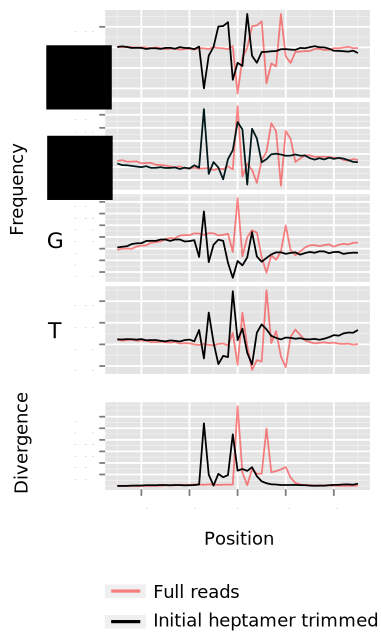
\includegraphics[width=0.35\textwidth]{fig/trimmed-freqs.pdf}
\end{center}



\section{Additional Kullback-Leibler Divergence Plots}

Below we plot the adjusted and unadjusted KL divergence plots, supplementing
those in the results section of the main paper.


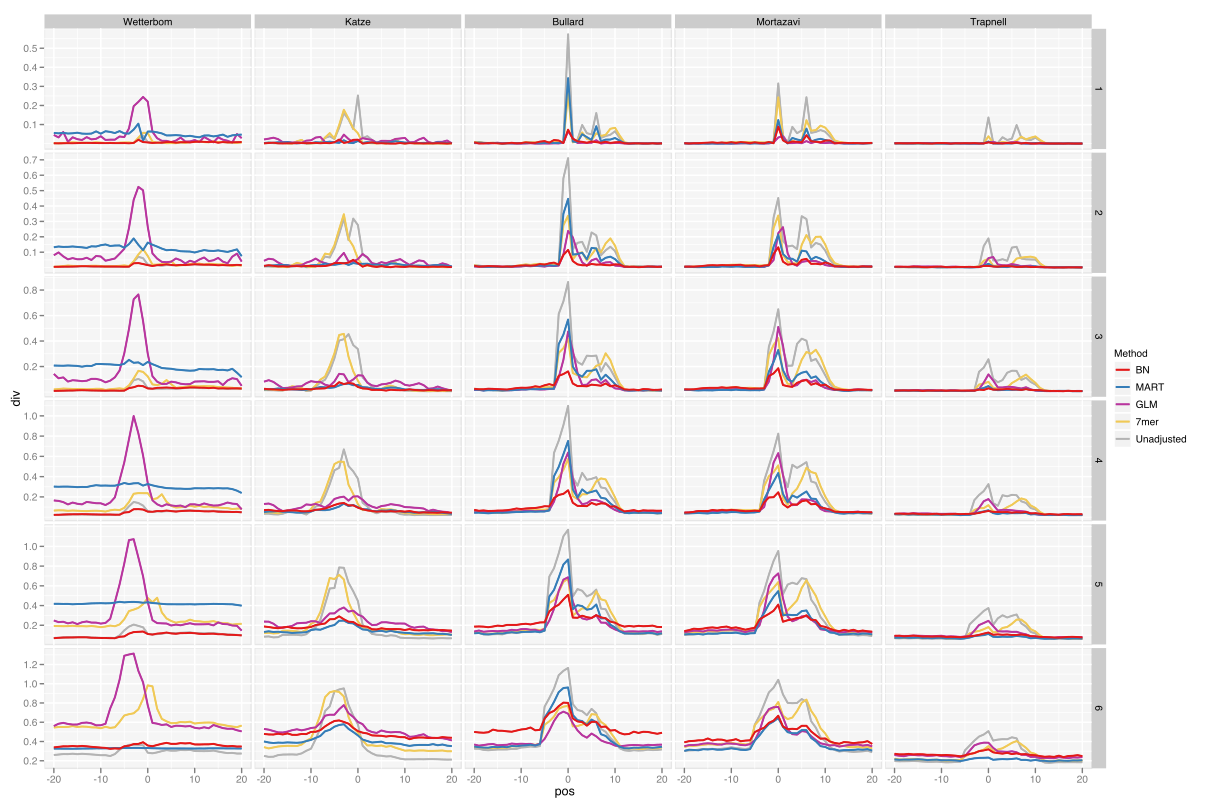
\includegraphics[width=\textwidth]{fig/kl-all.pdf}




\section{Runtime-Accuracy Trade-off}

Training our model on more reads results in more accurate estimation of bias,
but a longer training time. Here we investigate that trade-off by training our
model on progressively more reads from the Mortazavi data set. We use the
median pseudo-coefficient of determination ($R^2$) over exons selected for our
test set. Each point is additionally labeled with the time used to train the
model on one core of a 3Ghz Intel Xeon processor.

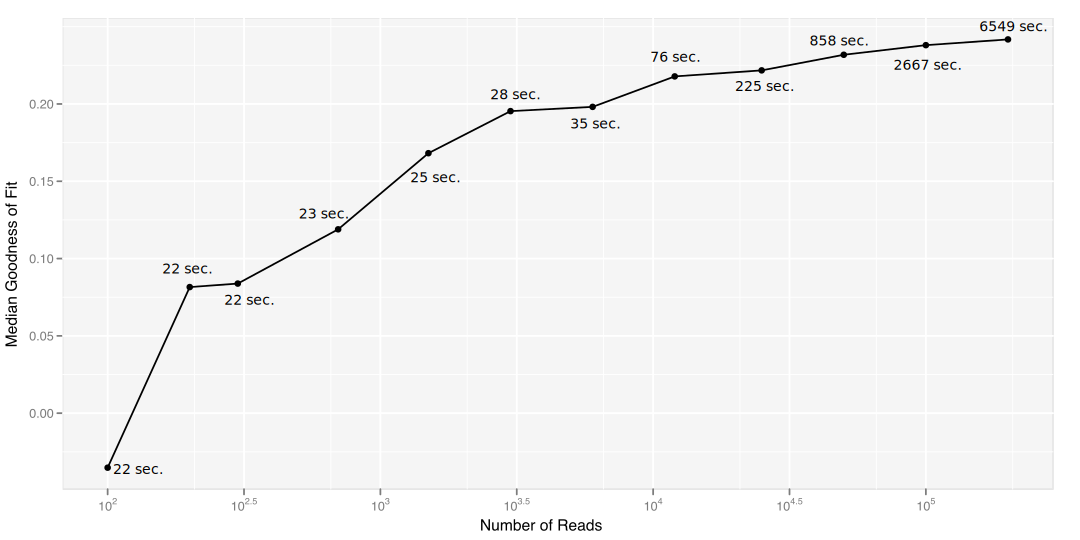
\includegraphics[width=\textwidth]{fig/pois-n.eps}


\section{ChIP-Seq}

Though the MART model \cite{Li2010} performed very well in several cases, ours
offers the advantage that no gene annotations are required for training.  In
RNA-Seq this is useful in applications of de-novo gene discovery, but it also
allows our method to be applied to ChIP-Seq and other short read data. Here we
examine one publicly available ChIP-Seq data set from Cao, et. al.
\cite{Cao2010}. Specifically, we used one run, with Sequence Read Archive
accession number SRR034831, containing 3,873,192 reads. These were mapped to the
reference genome using Bowtie \cite{Langmead2009}, resulting in 1,382,867
uniquely mapped reads, which were used for this analysis.

Measuring nucleotide frequencies, we find the bias to be significantly less
than that observed the RNA-Seq data sets we tested, but the data was by no means
unbiased.

\begin{center}
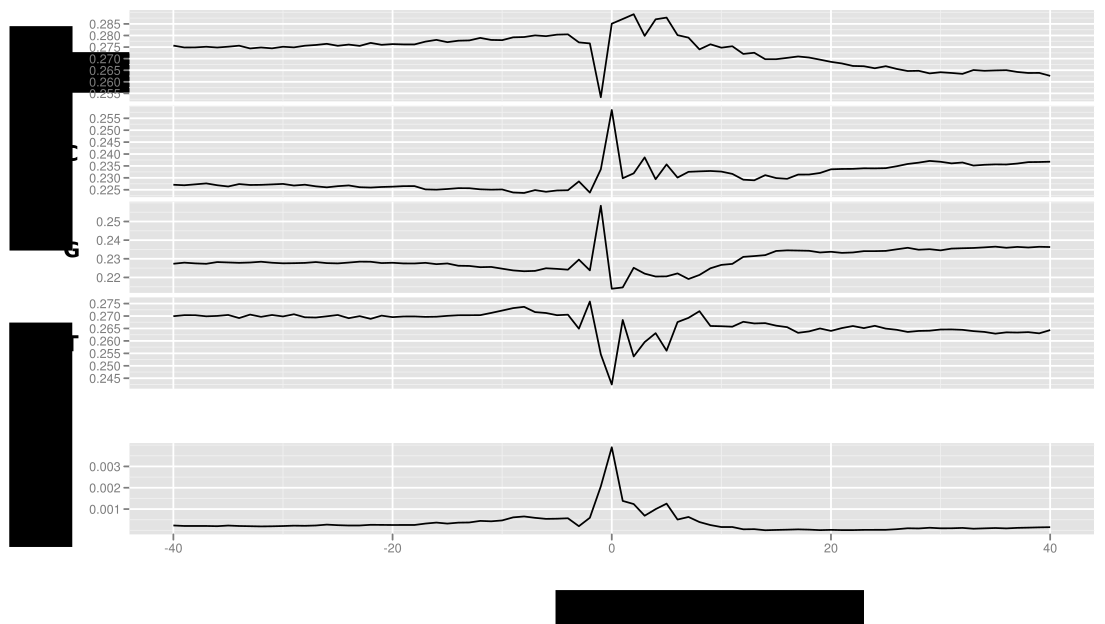
\includegraphics[width=0.7\textwidth]{fig/freqs_cao.pdf}
\end{center}

In the analysis of the RNA-Seq data, we used the assumption of continuous
transcription across annotated exons to evaluate the efficacy of the models, as
well as to train the GLM and MART models. Evaluating bias correction on ChIP-Seq
data necessitates dropping the Poisson regression test, as well as the GLM and
MART models from our comparison, which can not be applied to such data.

We did however repeat our analysis using the Kullback-Leibler divergence.
We used several variations of the method described by Hansen, et. al.,
\cite{Hansen2010}. ``7mer'' estimated the initial heptamer, ``Avg-7mer''
averages the initial two heptamers, and ``4mer'' averages the initial two 4mers.

We trained each method using reads from chromosomes 1--8. The
remaining chromosomes were segmented into 500nt bins, and the KL divergence was
sampled from the 50,000 segments with the highest read counts.

Below, we plot directly the positional KL divergence, computed in tho same
manner described in the Results section of the paper.

\begin{center}
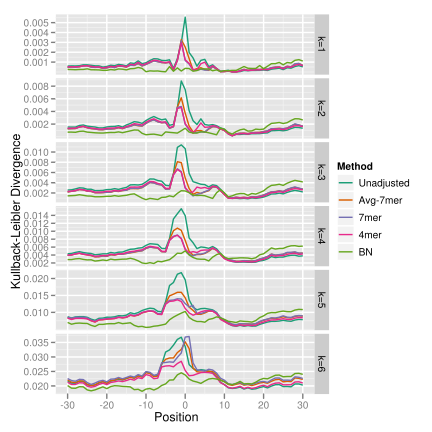
\includegraphics[width=0.5\textwidth]{fig/cao-kl.pdf}
\end{center}

We see that our method is effective at reducing the bias in this ChIP-Seq data.



\section{Variability Between Replicates}

Measuring differential expression or isoform switching is a primary application of
RNA-Seq. If the bias were inconsistent between replicates, it would call into
question the accuracy of such tests. In our experiments, we have observed the
bias to be mostly, but not entirely consistent between replicates. Below, we
plot the frequencies from the four runs in the Trapnell data set.

\begin{center}
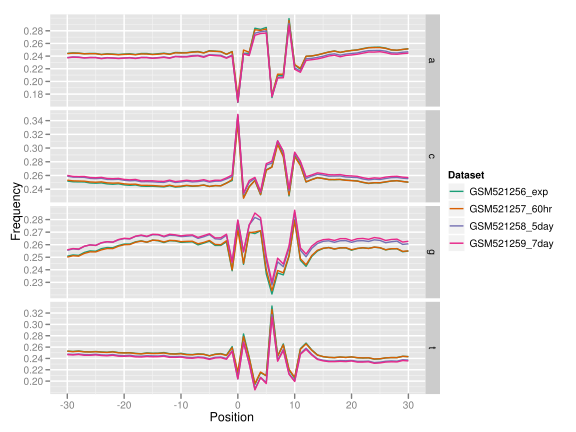
\includegraphics[width=0.5\textwidth]{fig/replicates.pdf}
\end{center}

Though we do not know if the variability is always minor, assuming this is so,
there remains the risk that the sequence bias would greatly effect the depth to
which a locus is sequenced, and thus the statistical significance of
differential expression tests. This would bias the discovery of differentially
expressed genes, but not the test itself.


\bibliographystyle{plain}
\bibliography{seqbias-paper}

\end{document}

